\documentclass[a4paper,12pt]{article}

% --- Tiếng Việt + mã UTF-8 ---
\usepackage[utf8]{inputenc}
\usepackage[T5]{fontenc}
\usepackage[vietnamese]{babel}

% --- Bố cục ---
\usepackage{geometry}
\geometry{top=2.5cm, bottom=2.5cm, left=3cm, right=2cm}

% --- Toán và bảng ---
\usepackage{amsmath}
\usepackage{amssymb}
\usepackage{booktabs}

% --- Hình ---
\usepackage{graphicx}
\graphicspath{{figures/}{../experiments/figures/}{../../}}

% --- Liên kết ---
\usepackage[hidelinks]{hyperref}

\setlength{\parskip}{3pt}

\begin{document}

% ===================== TRANG BÌA =====================
\begin{center}
ỦY BAN NHÂN DÂN THÀNH PHỐ HỒ CHÍ MINH\\
TRƯỜNG ĐẠI HỌC SÀI GÒN\\
KHOA TOÁN -- ỨNG DỤNG\\[0.6cm]


\includegraphics[width=4cm]{SGU-LOGO.png}\\[0.6cm]

{\Large\bfseries NHẬN DẠNG BIỂU CẢM KHUÔN MẶT\\[0.2cm]
TRÊN BỘ DỮ LIỆU FER2013 BẰNG MẠNG CNN}\\[0.8cm]

{\large Báo cáo bài tập môn Học sâu}\\[1.2cm]

\vfill

\begin{tabular}{rl}
Họ và tên: & Đinh Quang Minh \\
MSSV: & 3123580024 \\
Lớp: & DDU1231 \\
Ngành: & Khoa học dữ liệu \\
Giảng viên hướng dẫn: & TS. Đỗ Như Tài \\
\end{tabular}

\vfill

Học kỳ I, năm học 2026\\
TP. Hồ Chí Minh, tháng 11 năm 2026
\end{center}

\newpage

% ===================== 1. BÀI TOÁN =====================
\section*{1. Bài toán và dữ liệu}

Bài toán là phân loại một ảnh khuôn mặt $48\times48$ thành một trong 7 biểu cảm: giận, ghê tởm,
sợ hãi, vui, bình thường, buồn, ngạc nhiên. Bộ dữ liệu dùng trong bài là bản FER2013 trên Kaggle
(link gốc của cuộc thi không còn tải được nên dùng bản \texttt{msambare/fer2013}), đã tách sẵn
\textbf{28.709 ảnh train} và \textbf{7.178 ảnh test}, tất cả ở dạng ảnh xám $48\times48$.

Hai đặc điểm của dữ liệu ảnh hưởng trực tiếp đến cách đánh giá:

\begin{itemize}
  \item \textbf{Mất cân bằng mạnh}: lớp ghê tởm chỉ có 436 ảnh (1,5\%) trong khi lớp vui có 7.215
        ảnh (25,1\%), chênh 16,5 lần. Vì vậy nếu chỉ nhìn accuracy thì rất dễ bị đánh lừa — một mô
        hình đoán bừa ``vui'' đã được 25\%.
  \item \textbf{Nhiễu nhãn}: khi xem ảnh mẫu thấy có ảnh dính chữ watermark, ảnh tranh vẽ, và một
        số ảnh nhãn không khớp biểu cảm. Đây là lý do độ chính xác trên bộ này thường bão hoà quanh
        70\% dù mô hình rất mạnh.
\end{itemize}

\begin{figure}[h]
\centering
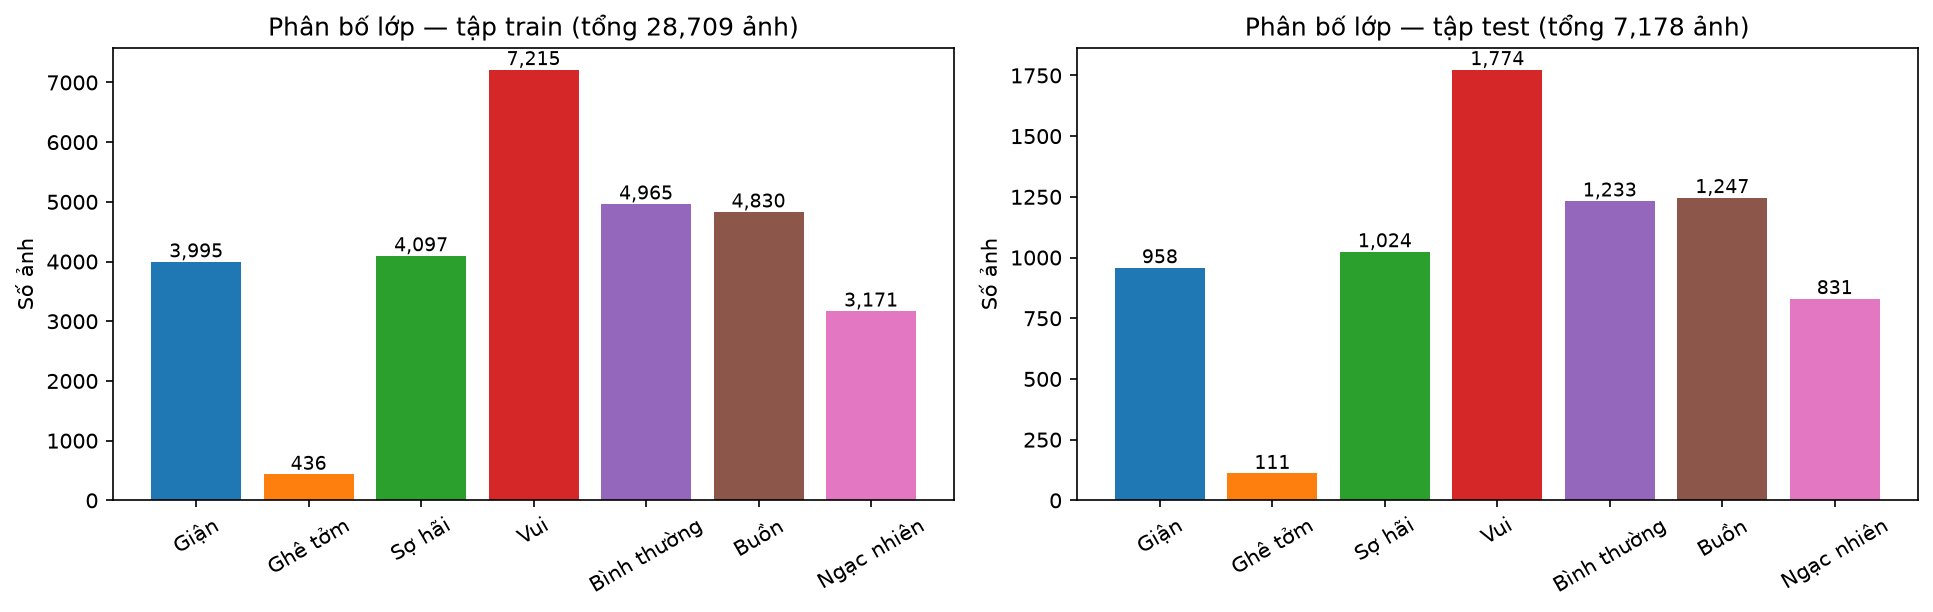
\includegraphics[width=0.95\textwidth]{eda_01_phan_bo_lop.png}
\caption{Phân bố số ảnh theo lớp ở hai tập. Lớp ghê tởm ít hơn lớp vui 16,5 lần.}
\end{figure}

Từ tập train, tôi tách stratified 10\% làm validation (25.838 ảnh train / 2.871 ảnh validation).
Tập test được giữ nguyên và chỉ dùng đúng một lần ở phần kết quả cuối.

\newpage

% ===================== 2. KIẾN TRÚC =====================
\section*{2. Kiến trúc mô hình}

Mạng cơ sở gồm các khối tích chập lặp lại theo công thức
$\text{Conv }3\times3 \to \text{BatchNorm} \to \text{ReLU} \to \text{MaxPool }2\times2$, sau đó là
Global Average Pooling, Dropout và một lớp fully-connected 7 đầu ra.

\begin{figure}[h]
\centering
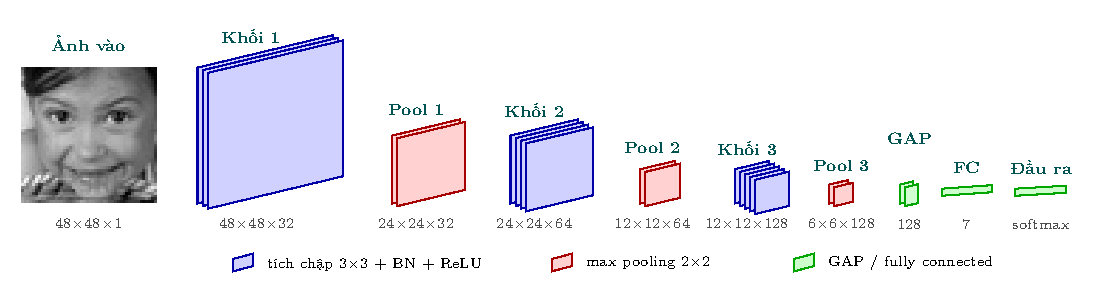
\includegraphics[width=\textwidth]{mo_hinh_baseline_3d.pdf}
\caption{Kiến trúc cơ sở: 3 khối tích chập (32-64-128), 93.799 tham số. Mô hình cuối dùng thêm
một khối thứ tư (128$\to$256), tổng 390.119 tham số.}
\end{figure}

Mô hình cuối được chọn sau phần thí nghiệm là bản \textbf{4 khối 32-64-128-256} (390.119 tham
số), huấn luyện với augmentation (lật ngang, xoay $\pm10^\circ$, dịch 8\%) và 40 epoch.

\newpage

% ===================== 3. THÍ NGHIỆM =====================
\section*{3. Các thí nghiệm so sánh}

Mỗi nhóm thí nghiệm chỉ đổi một biến so với baseline, các biến còn lại giữ nguyên. Mọi cấu hình
đều chạy 18 epoch, early stopping sau 6 epoch không cải thiện, và \textbf{chỉ nhìn validation} để
so sánh.

\begin{table}[h]
\centering
\caption{Kết quả 11 cấu hình so với baseline (validation accuracy, 18 epoch).}
\label{tab:thi-nghiem}
\small
\begin{tabular}{llrrr}
\toprule
Mã & Thay đổi so với baseline & Val acc & Chênh & Gap train--val \\
\midrule
BASE & 32-64-128, Adam $10^{-3}$ & 0,5385 & --- & $+0,022$ \\
A2   & 2 khối tích chập           & 0,3299 & $-20,9$ & $-0,002$ \\
A4   & 4 khối tích chập           & \textbf{0,5890} & $+5,0$ & $+0,324$ \\
B1   & mạng hẹp 16-32-64          & 0,4800 & $-5,9$ & $-0,001$ \\
B3   & mạng rộng 64-128-256       & 0,5730 & $+3,5$ & $+0,062$ \\
C1   & SGD momentum 0,9           & 0,5312 & $-0,7$ & $-0,006$ \\
C2   & AdamW                      & 0,5374 & $-0,1$ & $+0,020$ \\
C3   & Adam lr $10^{-4}$          & 0,4330 & $-10,6$ & $-0,006$ \\
D1   & có augmentation            & 0,5110 & $-2,8$ & $-0,010$ \\
D2   & dropout 0,5                & 0,5190 & $-2,0$ & $+0,029$ \\
D3   & class weight               & 0,4977 & $-4,1$ & $+0,007$ \\
D4   & augmentation + class weight & 0,4932 & $-4,5$ & $-0,001$ \\
\bottomrule
\end{tabular}
\end{table}

\begin{figure}[h]
\centering
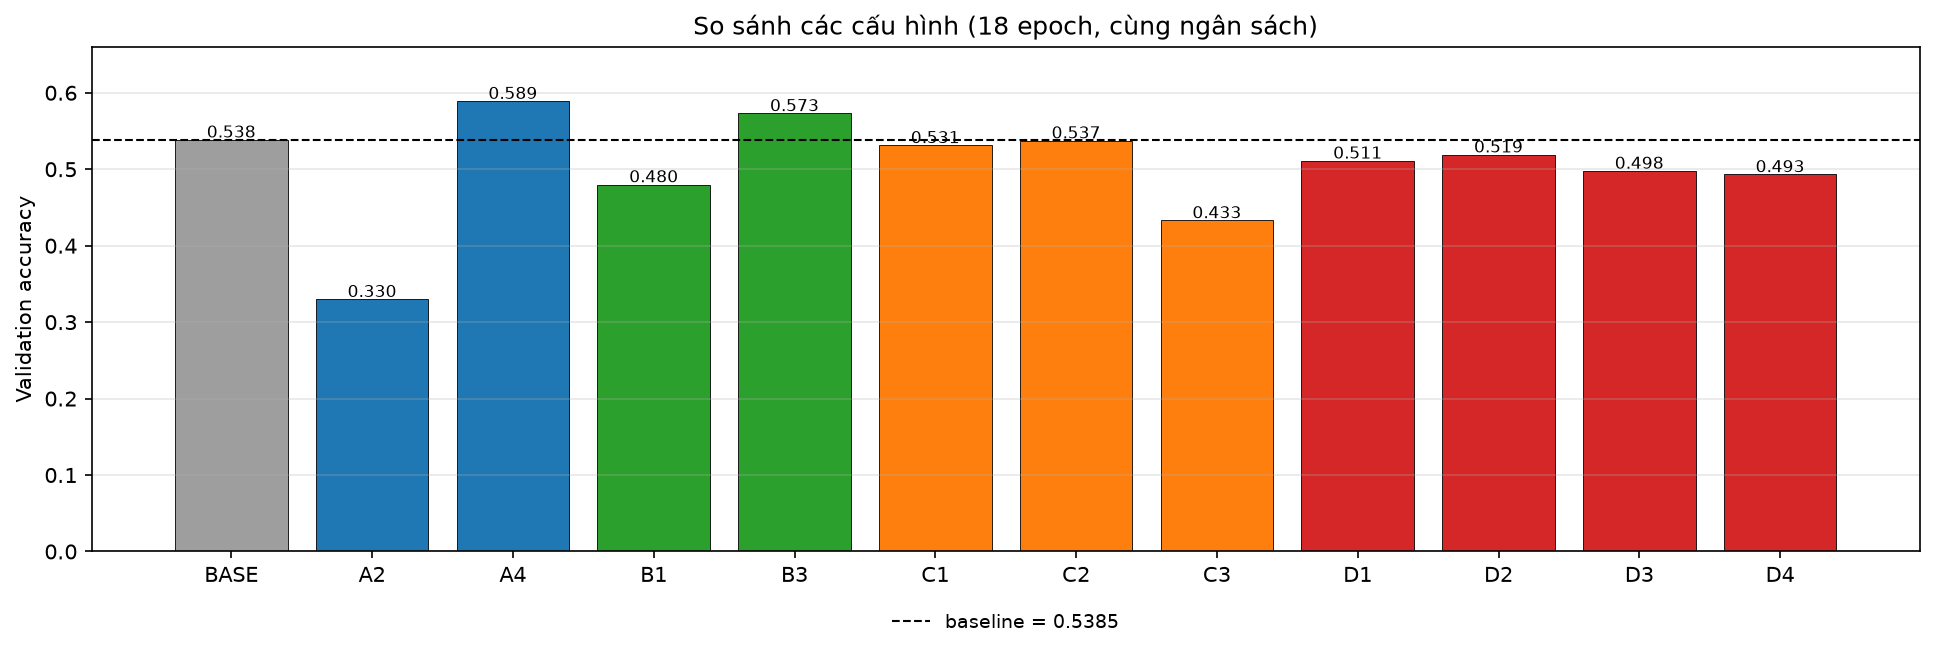
\includegraphics[width=\textwidth]{gd3_01_so_sanh_val_acc.png}
\caption{So sánh validation accuracy của 12 cấu hình. Đường nét đứt là mức baseline.}
\end{figure}

\newpage

\textbf{Nhận xét từng nhóm.}

\textbf{A -- độ sâu.} A2 chỉ đạt 0,33 và train cũng chỉ 0,328, tức mạng 2 khối \emph{không học
được gì đáng kể} (sau hai lần pooling chỉ còn lưới $12\times12$, GAP nén tiếp nên mất nhiều thông
tin không gian). A4 lên 0,589 nhưng train đạt 0,908 — quá khớp rất nặng. Hai kết quả này nói rằng
cần đủ độ sâu, nhưng thêm tầng mà không hãm quá khớp thì cũng không đi xa được.

\textbf{B -- độ rộng.} B3 hơn baseline 3,5 điểm nhưng tốn 1.531 giây so với 708 giây của A4, tức
A4 hiệu quả hơn trên mỗi giây. B1 thiếu tham số nên chỉ 0,480.

\textbf{C -- optimizer.} AdamW (0,5374) gần như trùng Adam (0,5385), SGD momentum (0,5312) chưa
hội tụ trong 18 epoch, còn lr $10^{-4}$ quá nhỏ (0,4330). Với bài này optimizer không phải đòn bẩy.

\textbf{D -- chống quá khớp.} Cả bốn cấu hình đều \emph{giảm} accuracy trong ngân sách 18 epoch.
Nhưng D1 có gap train--val xấp xỉ 0, nghĩa là augmentation đã chặn quá khớp đúng cách, chỉ có
điều 18 epoch là chưa đủ để hội tụ với bài toán bị làm khó hơn.

\newpage

% ===================== 4. KẾT QUẢ CUỐI =====================
\section*{4. Mô hình cuối và kết quả}

Từ hai kết luận trên, mô hình cuối là \textbf{A4 + augmentation, 40 epoch}, chạy 3 seed để có
trung bình và độ lệch chuẩn.

\begin{table}[h]
\centering
\caption{Kết quả 3 seed của mô hình cuối (validation).}
\begin{tabular}{lrrr}
\toprule
Seed & Epoch tốt nhất & Val accuracy & Val macro F1 \\
\midrule
42 & 36/40 & 0,6555 & 0,6087 \\
43 & 29/37 & 0,6444 & 0,5961 \\
44 & 37/40 & 0,6576 & 0,6138 \\
\midrule
Trung bình & & $\mathbf{0,6525 \pm 0,0071}$ & $0,6062 \pm 0,0091$ \\
\bottomrule
\end{tabular}
\end{table}

Độ lệch chuẩn chỉ 0,7 điểm, nhỏ hơn nhiều khoảng cách giữa các cấu hình ở bảng~\ref{tab:thi-nghiem},
nên các so sánh phía trên là đáng tin. Đáng chú ý: A4 ở 18 epoch có gap train--val là 0,324, còn
sau khi thêm augmentation và học 40 epoch gap chỉ còn 0,018 (train 0,675 / val 0,657) — tức
augmentation không làm mô hình yếu đi mà kéo nó về đúng mức.

Seed 44 được chọn (validation cao nhất) để đánh giá test một lần.

\begin{table}[h]
\centering
\caption{So sánh baseline và mô hình cuối trên tập test (7.178 ảnh).}
\begin{tabular}{lrr}
\toprule
 & Baseline & Mô hình cuối \\
\midrule
Accuracy & 0,5237 & \textbf{0,6503} \\
Macro F1 & 0,4278 & \textbf{0,6237} \\
Recall lớp ghê tởm & 0,00 & \textbf{0,53} \\
Recall lớp sợ hãi & 0,23 & 0,38 \\
\bottomrule
\end{tabular}
\end{table}

Mô hình cuối đạt \textbf{65,03\%} trên test, cách mốc tốt nhất của cuộc thi (69\% public) khoảng
4 điểm. Chi tiết theo lớp:

\begin{table}[h]
\centering
\caption{Precision / recall / F1 từng lớp của mô hình cuối trên test.}
\small
\begin{tabular}{lrrrr}
\toprule
Lớp & Precision & Recall & F1 & (F1 baseline) \\
\midrule
Giận        & 0,580 & 0,551 & 0,565 & 0,410 \\
Ghê tởm     & 0,641 & 0,531 & 0,581 & 0,000 \\
Sợ hãi      & 0,537 & 0,385 & 0,448 & 0,274 \\
Vui         & 0,845 & 0,861 & \textbf{0,853} & 0,749 \\
Bình thường & 0,587 & 0,627 & 0,606 & 0,514 \\
Buồn        & 0,507 & 0,582 & 0,542 & 0,387 \\
Ngạc nhiên  & 0,746 & 0,795 & 0,770 & 0,660 \\
\bottomrule
\end{tabular}
\end{table}

\begin{figure}[h]
\centering
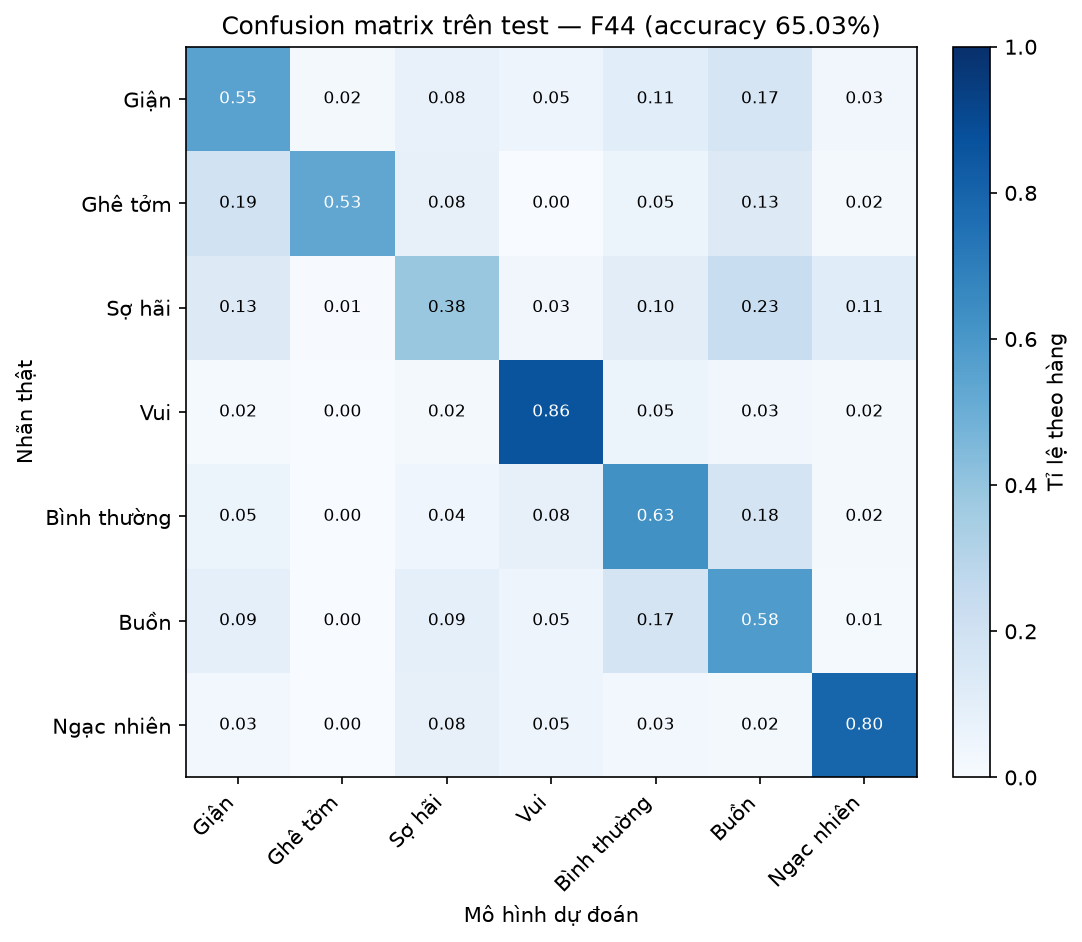
\includegraphics[width=0.85\textwidth]{gd4_01_confusion_test.png}
\caption{Confusion matrix chuẩn hoá theo hàng (mỗi hàng là một lớp thật). Đường chéo là recall.}
\end{figure}

\newpage

Ba lớp dễ lẫn nhất là sợ hãi -- buồn -- bình thường, đúng như dự đoán từ phần dữ liệu. Năm cặp
nhầm nhiều nhất: sợ hãi $\to$ buồn 23,3\%; ghê tởm $\to$ giận 18,9\%; bình thường $\to$ buồn
17,8\%; buồn $\to$ bình thường 17,2\%; giận $\to$ buồn 16,7\%. Lớp buồn xuất hiện trong 4/5 cặp,
tức nó đóng vai trò ``lớp hút'' khi mô hình phân vân.

Một kết quả phụ đáng ghi: bản có \textbf{class weight} (cùng seed 42) chỉ đạt 0,6371 và macro F1
0,5869, đều \emph{thấp hơn} bản không dùng (0,6555 / 0,6087). Khi mô hình đã đủ năng lực và có
augmentation, lớp hiếm tự học được, nên ép trọng số chỉ làm lệch dự đoán về phía lớp hiếm và mất
điểm ở các lớp phổ biến.

\newpage

% ===================== 5. TRỰC QUAN =====================
\section*{5. Trực quan hoá bộ lọc và bản đồ đặc trưng}

\begin{figure}[h]
\centering
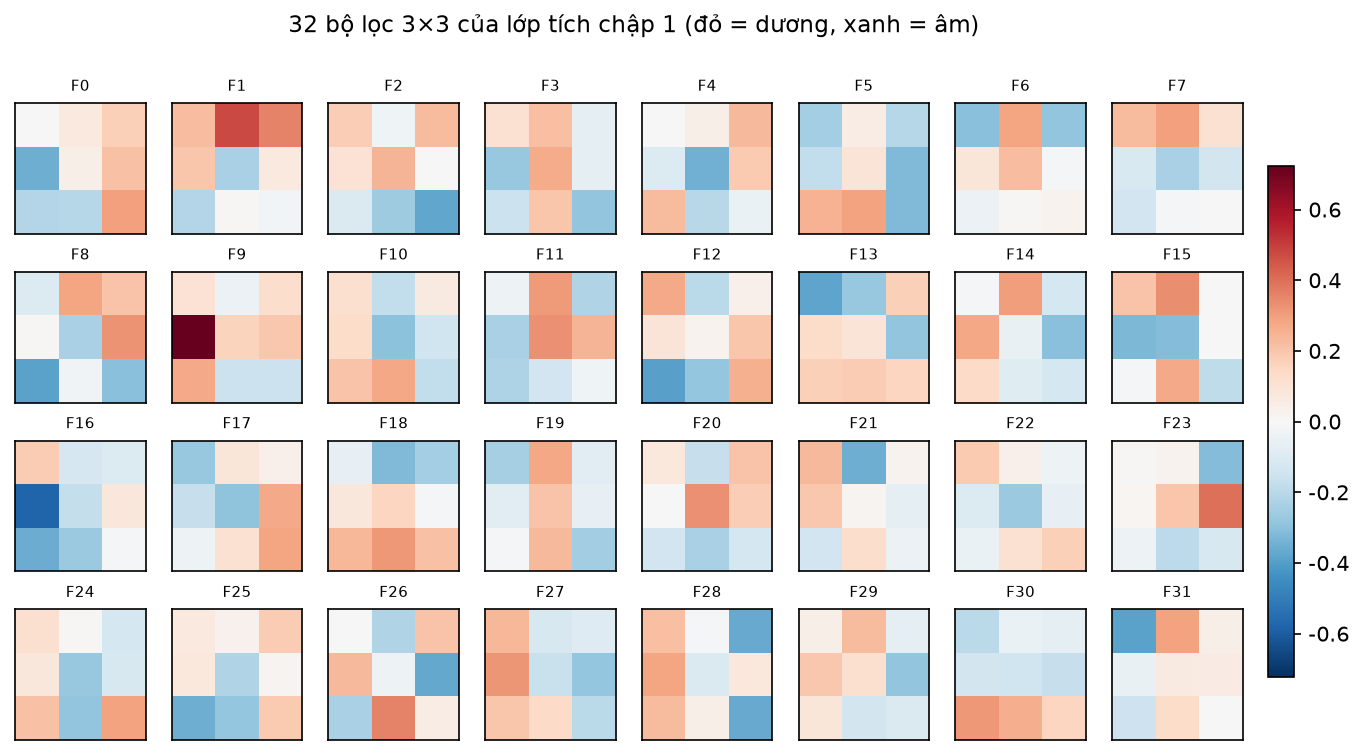
\includegraphics[width=\textwidth]{gd5_01_filter_conv1.png}
\caption{32 bộ lọc $3\times3$ của lớp tích chập 1 (đỏ = trọng số dương, xanh = âm).}
\end{figure}

Bộ lọc lớp 1 có hai kiểu rõ rệt: phần lớn là \textbf{hai vùng đối lập} (nửa đỏ, nửa xanh) tương
đương bộ dò cạnh theo hướng; một số dồn trọng số vào \textbf{một điểm} để dò đốm sáng/tối cục bộ.
Năng lượng theo 8 vị trí của ô $3\times3$ gần như bằng nhau (0,15--0,19), nên không filter nào
khoanh vùng một góc riêng.

\begin{figure}[h]
\centering
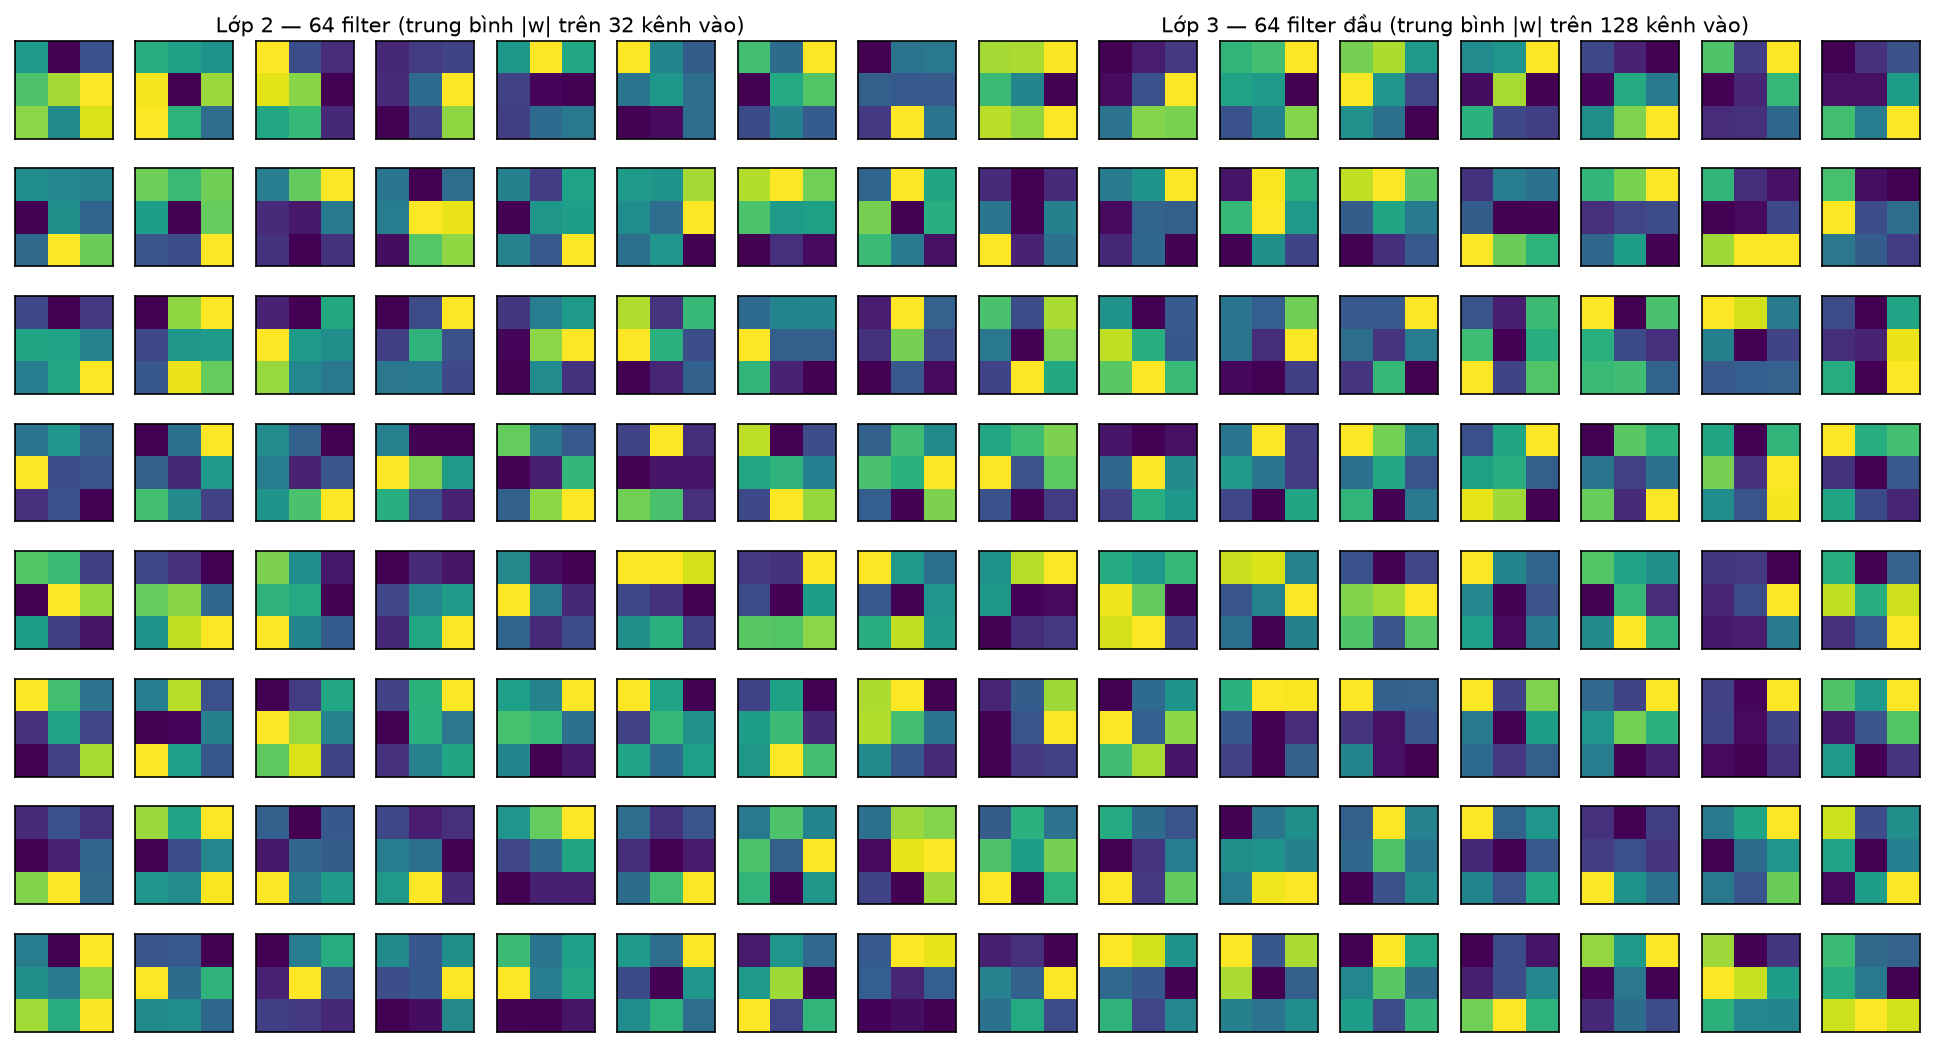
\includegraphics[width=\textwidth]{gd5_02_filter_conv23.png}
\caption{Bộ lọc lớp 2 (64 filter, trung bình $|w|$ trên 32 kênh vào) và 64 filter đầu của lớp 3
(trung bình trên 128 kênh vào).}
\end{figure}

Hai lớp sâu hơn có năng lượng trung bình gần như trùng nhau (0,0755 và 0,0748) và không filter nào
vượt 2 lần mức trung bình — mạng phân bố đều chứ không dành riêng một nhóm filter ``chuyên gia''.

\begin{figure}[h]
\centering
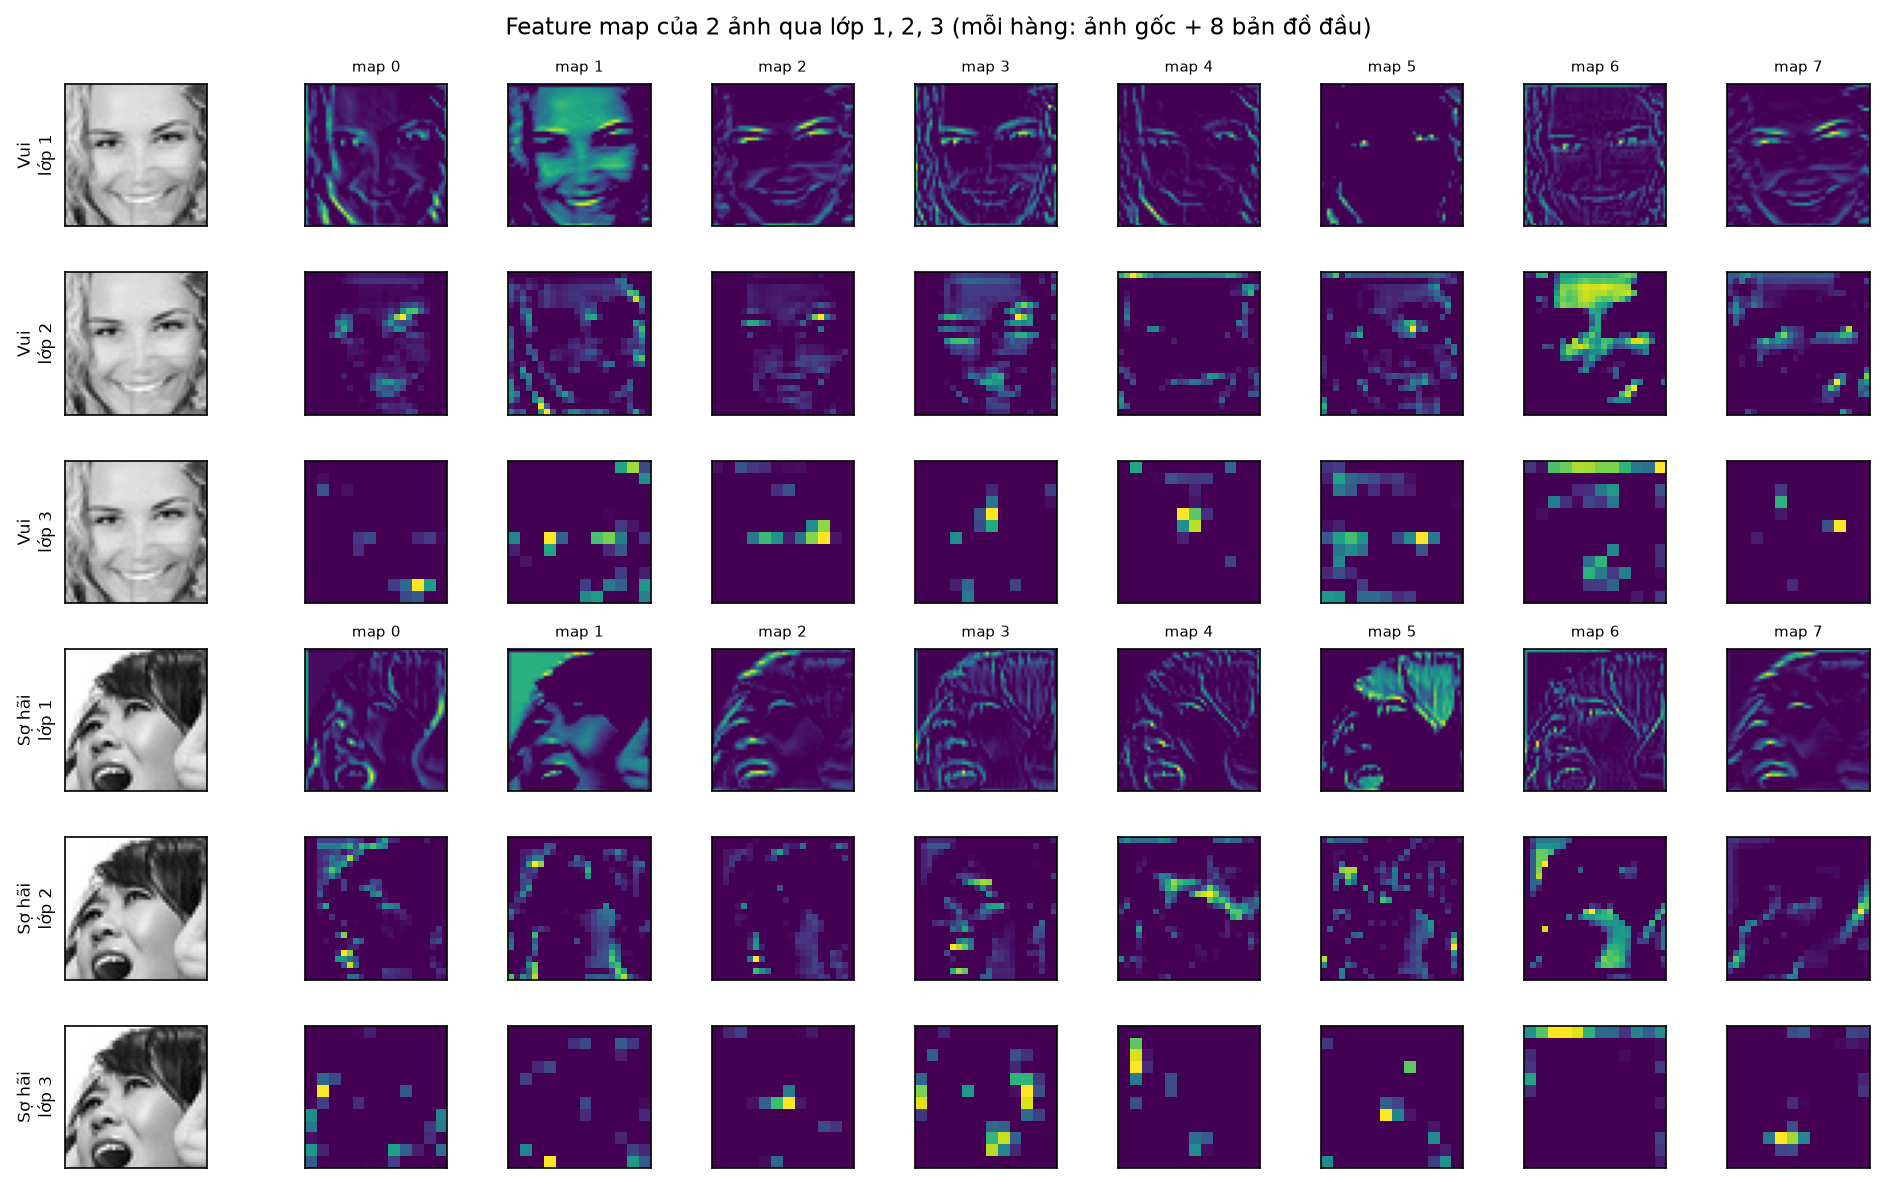
\includegraphics[width=\textwidth]{gd5_03_feature_maps.png}
\caption{Bản đồ đặc trưng của một ảnh ``vui'' và một ảnh ``sợ hãi'' qua lớp 1, 2, 3.}
\end{figure}

Bản đồ đặc trưng cho thấy mức trừu tượng tăng dần: lớp 1 ($48\times48$) vẫn nhận ra khuôn mặt với
mắt và miệng sáng lên; lớp 2 ($24\times24$) chỉ còn các đốm ở mắt, lỗ mũi, khoé miệng; lớp 3
($12\times12$) gần như không còn hình dạng, trong khi số kênh tăng từ 32 lên 128. Ảnh ``vui'' kích
hoạt mạnh vùng má và khoé miệng, ảnh ``sợ hãi'' kích hoạt vùng mắt và miệng mở rộng — khác biệt
có nhưng mong manh, khớp với việc mô hình vẫn nhầm sợ hãi thành buồn 23\% số lần.

\newpage

% ===================== 6. MÃ NGUỒN =====================
\section*{6. Tóm tắt mã nguồn}

Toàn bộ chương trình viết bằng PyTorch, chạy được trên CPU. Cấu trúc thư mục:

\begin{center}
\small
\begin{tabular}{ll}
\toprule
Đường dẫn & Nội dung \\
\midrule
\texttt{notebooks/cnn\_fer.ipynb} & toàn bộ pipeline: nạp dữ liệu, chia tập, định nghĩa mô hình, \\
 & huấn luyện, 11 thí nghiệm, mô hình cuối, đánh giá, trực quan \\
\texttt{notebooks/EDA.ipynb} & khảo sát dữ liệu (phân bố lớp, ảnh mẫu, độ sáng) \\
\texttt{experiments/} & \texttt{runs.csv}, \texttt{final\_seeds.csv}, \texttt{model\_log.md}, \\
 & \texttt{logs/*\_history.csv}, \texttt{models/*.pt} \\
\texttt{report/} & nguồn LaTeX và PDF của báo cáo này \\
\bottomrule
\end{tabular}
\end{center}

Chạy lại toàn bộ notebook bằng một lệnh:

\begin{center}
\texttt{jupyter nbconvert --to notebook --execute --inplace notebooks/cnn\_fer.ipynb}
\end{center}

Notebook có cơ chế chạy tiếp: cấu hình nào đã có kết quả trong \texttt{runs.csv} hoặc đã có file
trọng số trong \texttt{experiments/models/} thì tự bỏ qua, nên không phải huấn luyện lại từ đầu.
Toàn bộ seed đều cố định ($SEED = 42$) để kết quả tái lập được.

\newpage

% ===================== 7. KẾT LUẬN =====================
\section*{7. Kết luận}

Với một mạng CNN tự viết, chạy trên CPU, mô hình đạt \textbf{65,03\%} trên tập test — chỉ kém mốc
tốt nhất của cuộc thi khoảng 4 điểm, và hơn baseline 12,7 điểm accuracy, 19,6 điểm macro F1.

Yếu tố cải thiện lớn nhất không phải kiến trúc hay optimizer mà là \textbf{ngân sách huấn luyện đi
kèm augmentation}: cùng bộ 4 khối, tăng từ 18 lên 40 epoch và thêm augmentation đưa validation từ
0,589 lên 0,6525, đồng thời kéo khoảng cách train--validation từ 0,324 xuống 0,018. Dung lượng mô
hình là yếu tố quan trọng thứ hai; optimizer gần như không tạo khác biệt; còn class weight và
dropout lớn đều làm giảm chất lượng trên bộ dữ liệu này.

Hạn chế còn lại nằm ở dữ liệu: ảnh $48\times48$ quá nhỏ và nhãn có nhiễu, khiến ba lớp sợ hãi --
buồn -- bình thường vẫn lẫn nhau. Hướng cải thiện hợp lý tiếp theo là làm sạch nhãn, hoặc dùng
kiến trúc mạnh hơn (ResNet nhỏ) cùng augmentation mạnh hơn, thay vì tiếp tục tăng số tầng.

\end{document}
